
\chapter{Thomas's Tangles}
A recently released book Teaching Computing Unplugged in Primary Schools  edited by Helen Caldwell (University of Northampton) and Neil Smith (Open University) has a number of interesting chapters by authors who are passionate about how computing is taught in schools. The central theme is unplugged activities, without using computers, but still teach the fundamental of computational thinking.

Ok, confession time. I co-wrote, along with Katharine Childs (Raspberry Pi Foundation), Chapter 3 Artists so I am biased here, but I believe in the central theme of Unplugged Computing. Computing, and Computational Thinking in general,  is not just about programming and using a computer (though using computers and  programming are vitally important to Computing) but it is also about many other things including problem-solving, being creative and working collaboratively.

Chapter 3 is about linking these computational thinking ideas to produce visual art, by applying computing principles including  repetition, following and refining algorithms, and abstraction. The chapter also looks, how these links have already being made, with examples such Sol Le Witt where not all the work that was produced by the artist himself, but some by others following his written instructions - in other words an algorithm. There is even a game Thomas's Tangles

The other chapters make links with areas such as Robots, Musicians, Explorers, Magicians, Gamers, Cooks and Scientists.

\sectionn{Tools we can use}

A sequence of instructions
\begin{lstlisting}
Find the lid of a bottle
Turn lid of the bottle until lid comes off
\end{lstlisting}

A loop to repeat a sequence until something we define happens or even for ever. So our instruction "Turn lid of the bottle until lid comes off" might be changed to get a certain sequence of instructions to be repeated. I am going use indenting to show what is in the loop (bit that repeats).
\begin{lstlisting}
hold the bottle
Repeat until lid comes off
   turn the lid 45 degrees anti-clockwise
   release lid hand 
   move lid back starting position
   check does the lid come off
\end{lstlisting}

Our last tool is a test (conditional statement) where we can what happens based on what the outcome of the test is, Again I i am going to use indenting to show what belong togther. In the previous 'code' we had a line saying "check does the lid come off" which was two outcome if does or it doesn't,

\begin{lstlisting}
if check does the lid come off == yes
   pull the lid vertical 10 cm
   stop the algorithm
\end{lstlisting}

So lets put all of these together
\begin{lstlisting}
Find the lid of a bottle
hold the bottle
Repeat until lid comes off
   turn the lid 45 degrees anti-clockwise
   release lid hand 
   move lid back starting position
   if check does the lid come off == yes
     pull the lid vertical 10 cm
     stop the algorithm
\end{lstlisting}

So know we have a starting point for a routine/algorithm for opening a bottle. 

\section{Make your own game}
This activity is about computing ideas to build a paper-based game, to create pictures by creating and then following routines (Algorithms) We are going to use the three tools to make the games. 

Goal 1: At the end of the session you have produce a paper-based games instructions that use dice, pens and paper to produce random drawings (see below). The instructions should look a bit like the bottle opening routine 

\begin{figure}
    \centering
    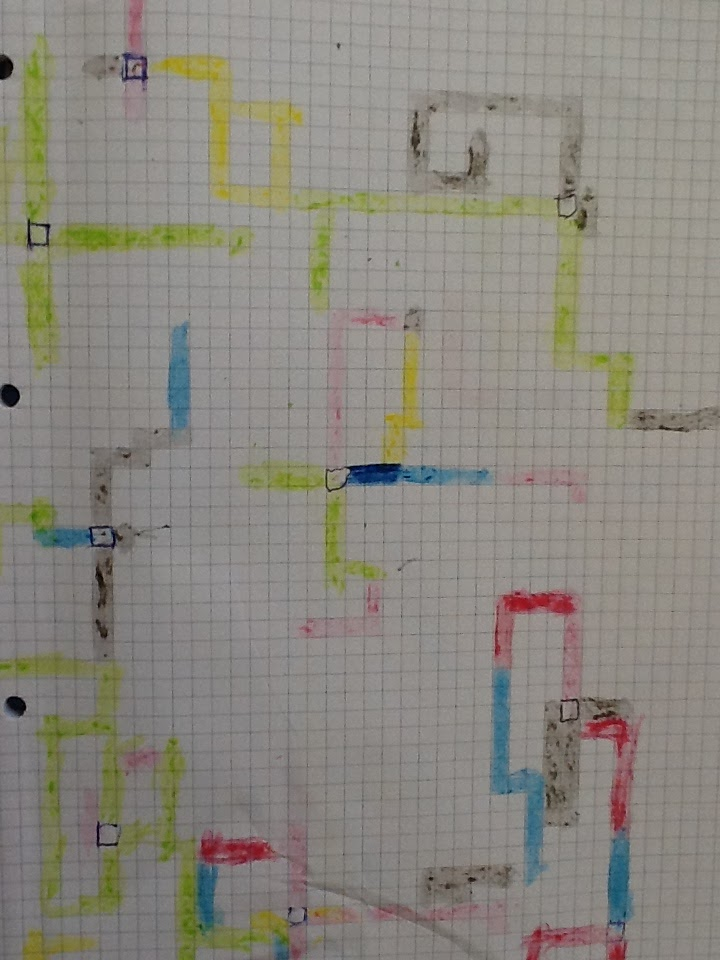
\includegraphics[width=10cm]{chapters/chapterCT1/figures/tt1.JPG}
    \caption{Thomas' Tangles}
    \label{fig:ThomasTangles1}
\end{figure}

Goal 2: You have tested some one else's games and constructively feedback 

You have two dice, some pens and paper.

First 20 minutes
Working in groups of 2-3 people
Develop your games and produce the instructions

Remaining 
Swap your game with another group and each try their game.
Pass back constructive feedback to the other group.

Don't panic: In case of emergency in the next section there is an example, please build your own.


\section{Thomas Tangles}
This simplifies the algorithm Thomas' Tangles (named after my son who helped develop it) in Chapter 3 of the book discussed in http://compuationalthinking.blogspot.co.uk/2016/11/how-to-be-unplugged-artist.html

Using crayons, pencils or pens, we are going to follow an algorithm to create a random drawing. This could be done in pairs and you will need squared paper. 

Person A: Rolls the dice and reads out the instructions - their role is to roll the dice, interpret the algorithm and tell the 'robot' what to do.

Person B: Is the ‘robot carrying out the instructions'. The lines are solid blocks of colour so move four squares does also mean colour in the squares between the start and finish in the direction of movement.

\begin{figure}
    \centering
    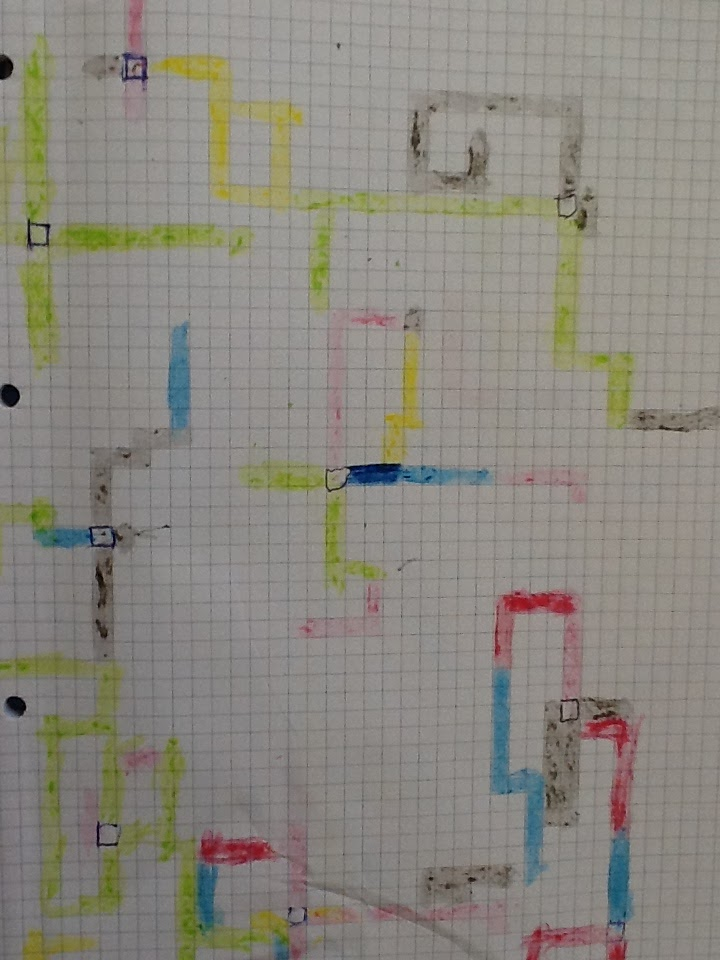
\includegraphics[width=10cm]{chapters/chapterCT1/figures/tt1.JPG}
    \caption{Thomas' Tangles}
    \label{fig:ThomasTangles1}
\end{figure}

When a new central square is needed the roles of A and B swap (so A is the ‘robot’ and B rolls the dice and reads out the instruction). The roles keep swapping.

\begin{lstlisting}
Start from a random square – call it the centre square
Repeat until end of game
If die roll = 1
  Roll die for number of moves
 move die roll number of steps up the page
If die roll = 2
  Roll die for number of moves
  move die roll number of steps down the page
If die roll = 3
  Roll die for number of moves
  move die roll number of steps to the left 
If die roll = 4
  Roll die for number of moves
  move die roll number of steps to the right
If die roll = 5
  Roll die
  If die = 1 change colour to Red
  If die = 2 change colour to Blue
      If die = 3 change colour to Black
  If die = 4 change colour to Green
  If die = 5 change colour to Orange
  If die = 6 change colour to Yellow
If die roll = 6
           Roll die
  Return to current centre square
                If the second die roll=6
                   randomly select new centre square
     if block is off the page
                randomly select new centre square
\end{lstlisting}

The Scratch version can be here \url{https://scratch.mit.edu/projects/135816631/} if you wish to see the code.

